\section{\"Ubertragung des Lastenhefts in Wireframes}

Bei der Bearbeitung des Projekts wurde entschieden, nach der Lastenheftanalyse, zuerst die gesamte GUI nach der Aufgabenstellung des Lastenhefts zu modelieden. Durch diese Vorgehensweise wird schneller ersichtlich welche Android-Komponenten genau ben\"otigt werden und wie sie zu implementieren sind.

F\"ur die Modellierung der Wireframes wurde das Mockup-Tool WireframeSketcher verwendet, welches \"ahnlich wie \ac{ADT} auch ein Eclipse-Plugin ist. 

Nach einer ersten Erstellung der Wireframes wird eine Evaluierung mit Hilfe der Kameraden der Freiwilligen Feuerwehr Rastenberg stattfinden, bei der eventuelle Schwachstellen oder Verbesserungen diskutiert werden sollen.

\subsection{Die Wireframes}
  
\begin{wrapfigure}{l}{10cm}
\vspace{-13pt}
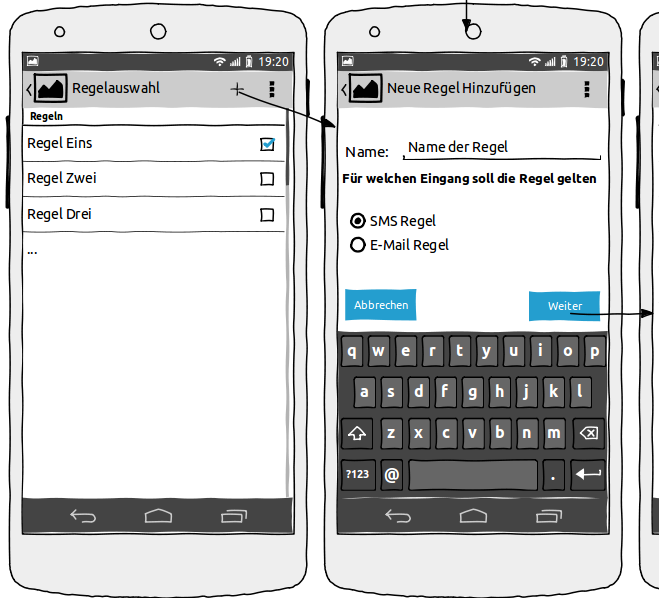
\includegraphics[width=10cm]{Bilder/StartBildschirm.png}
\caption{Wireframe des StartBildschirms mit der Erstellung einer Regel}
\label{Wireframe StartBildschirm}
\vspace{-10pt}
\end{wrapfigure}
Im Bild \ref{Wireframe StartBildschirm} sind die ersten zwei Wireframes zu sehen. Im linken Frame ist der StartBildschirm der App abgebildet, welcher bei Start der App angezeigt werden soll. Hier hat der Nutzer eine \"Ubersicht \"uber alle seine Regeln, welche mit Hilfe der Checkboxen rechts aktiviert und deaktiviert werden k\"onnen, wie des das Lastenheft nach LF70 verlangt. In der oberen Men\"uleisten ist zum einen ein Plus-Symbol, sowie das standard Android-Symbol f\"ur das Activity abh\"angige Popupmen\"u.

Tippt der Nutzer nun auf das Plus-Symbol, gelangt er zu einer neuen Activity (im Bild \ref{Wireframe StartBildschirm} rechts), mit der er eine neue Regel erzeugen kann.
Die neue Activity verlangt zum einen eine Namen f\"ur die Regel, sowie eine Angabe, ob es sich bei der Regel um eine SMS-Regel oder eine E-Mail-Regel handelt, was \"uber die Radiobutton unter dem Textfeld geschieht.

Im unteren Teil der Activity hat der Nutzer zwei Button, zum einen um die Aktion abzubrechen und zum anderen einen Button um weitere Regeleinstellungen vorzunehmen.
Beim bet\"atigen des Weiter-Button gelangt der Nutzer auf eine weitere Activity welche im Bild \ref{Wireframe Regeluebersicht} dargestellt ist.

Das Bild \ref{Wireframe Regeluebersicht} zeigt die n\"achsten Wireframes. Im linken Frame ist die \"Uberischt \"uber alle Einstellungsm\"oglichkeiten einer Regel zu finden. Tippt der Nutzer nun auf eine dieser Auswahlm\"oglichkeiten, so gelangt er zur jeweiligen Activity. Im weiteren Verlauf werden alle aufgef\"uhrten Activitys dargestellt und genauer erl\"autert.
Alle nun folgenden Activitys sehen gleich aus, egal ob es sich nun um eine SMS-Regel oder E-Mail-Regel handelt.

Wurde die Absenderauswahl gew\"ahlt, so gelangt man zu einer Activity welche es erm\"oglicht einen Absender einzugeben. Hier hat der Nutzer die Wahl, ob er selbst eine Nummer hinzuf\"ugt, oder ob er \"uber den Button "`Auswahl aus Kontakten"' einen Kontakt w\"ahlt. Wird nun dieser Button get\"atigt, so gelangt man zu einem Content Provider (im Bild \ref{Wireframe Regeluebersicht} rechts dargestellt), welcher alle Kontakte auflistet. 

Hier ist es m\"oglich einen Kontakt \"uber die Suchleite zu finden, oder einfach nach unten zu scrollen. Wird ein Kontakt ausgew\"ahlt, so gelangt der Nutzer automatisiert zur Absenderauswahl zur\"uckt und der gew\"ahlte Kontakt wird ins Absender-Feld eingetragen.

Je nachdem, ob es sich um eine SMS- oder E-Mail-Regel handelt, wird die Telefonnummer beziehungsweise die E-Mail-Adresse eingetragen.

Ist die Auswahl vollendet, gelangt der Nutzer \"uber den Speichern-Button zur\"uck zur linken Activity wo er weitere Einstellungen vornehmen kann.
\begin{figure}[!ht]
\centering
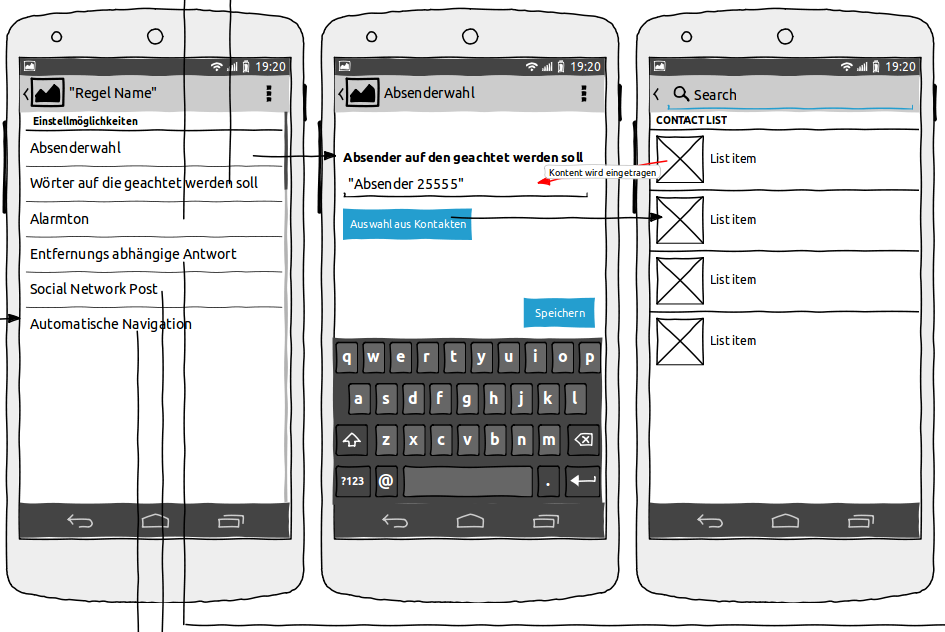
\includegraphics[width=16cm]{Bilder/WireframeRegeluebersicht.png}
\caption{Wireframe der Regel\"ubersicht und der Absenderauswahl}
\label{Wireframe Regeluebersicht}
\centering
\end{figure}

\newpage

 
\begin{wrapfigure}{l}{10cm}
\vspace{-13pt}
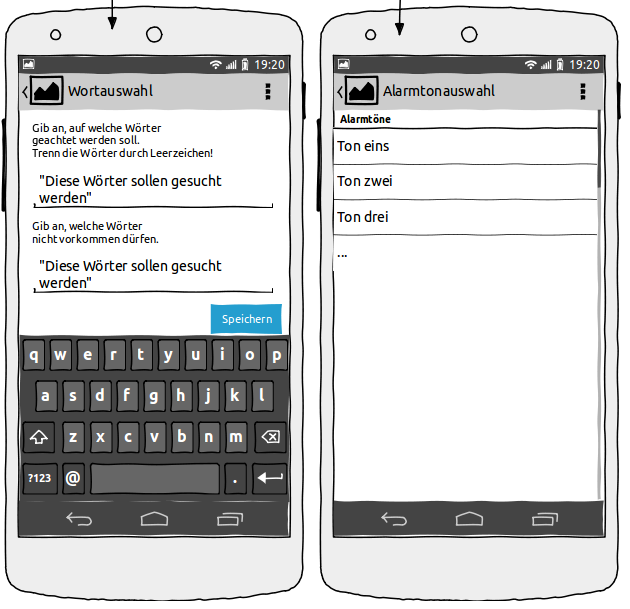
\includegraphics[width=10cm]{Bilder/WireframeWortwahl.png}
\caption{Wireframe der Wortauswahl und der Alarmtonwahl}
\label{Wireframe Wortauswahl}
\vspace{-20pt}
\end{wrapfigure}
Tippt der Nutzer nun auf die Wortauswahl (im Bild \ref{Wireframe Regeluebersicht} links) so gelangt er auf eine Activity, welche es ihm erm\"oglicht Schl\"usselw\"orter auszuw\"ahlen. Im Bild \ref{Wireframe Wortauswahl} ist die Activity mit der Schlagwortauswahl links dargestellt. 

Der Nutzer hat nun den M\"oglichkeit Schlagw\"orter zu w\"ahlen, welche vorkommen m\"ussen und welche nicht enthalten sein d\"urfen. Sind beide Felder leer, so reicht es aus, das eine Nachricht vom Absender eingeht, um einen Alarm auszul\"o\ss{}en.

Sollten die Felder einen Inhalt haben, so wird die Nachricht auf diese geparst. Sollten die Informationen zutreffen, das hei\ss{}t sind alle W\"orter vorhanden beziehungsweise sind ausgeschlossene W\"orter nicht vorhanden wird ein Alarm abgesetzt. 

Die einzelnen W\"orter m\"ussen wie in der Activity beschrieben durch ein Leerzeichen getrennt werden.

In der rechten Activity ist die Tonauswahl dargestellt, hier hat der Nutzer die M\"oglichkeit einen Alarmton auszuw\"ahlen, welcher beim zutreffen der Regel abgespielt wird. In der Auswahl sind die standard T\"one des Smartphones und die mit der App mitgelieferten T\"one zu finden.

Im Bild \ref{Wireframe Antwort} ist in der linken Activity die Erstellung der automatisierten Antwort dargestellt. Wie schon im Bild \ref{Wireframe Regeluebersicht} ist die Empf\"angerauswahl wieder manuell und \"uber einen Content Provider geregelt. Im Textfeld darunter kann der Nutzer eine Nachricht eingeben, welche automatisch gesendet wird sollte beim Empfangen einer Alarmnachricht eine gewisse weite zum Ger\"atehaus \"uberschritten sein.

Die Entfernung kann der Nutzer nat\"urlich auch ausw\"ahlen, und zwar \"uber eine Listenauswahl, welche im unteren Teil der Activity zu finden ist. Um alle informationen zu Speichern gibt es auch in dieser Activity wieder einen Speichern Button.

In der rechten Activity im Bild \ref{Wireframe Antwort} ist die Voreinstellung f\"ur einen Facebookpost zu treffen. Der Nutzer kann einen standard Text angeben, der beim erhalt einer Nachricht automatisch auf Facebook gepostet wird. Auch ist es m\"oglich \"uber die Checkbox den Nachrichtentext mit an den Post anzuh\"angen. Um einen Facebookpost zu ver\"offentlichen muss entweder die App der Facebook AG auf dem Ger\"at installiert sein, oder die Facebook API in das Projekt eingebaut werden. Welcher weg der proaktikablere ist, wird im Kapitel ????? genauer erl\"autert.
\begin{figure}[!ht]
\centering
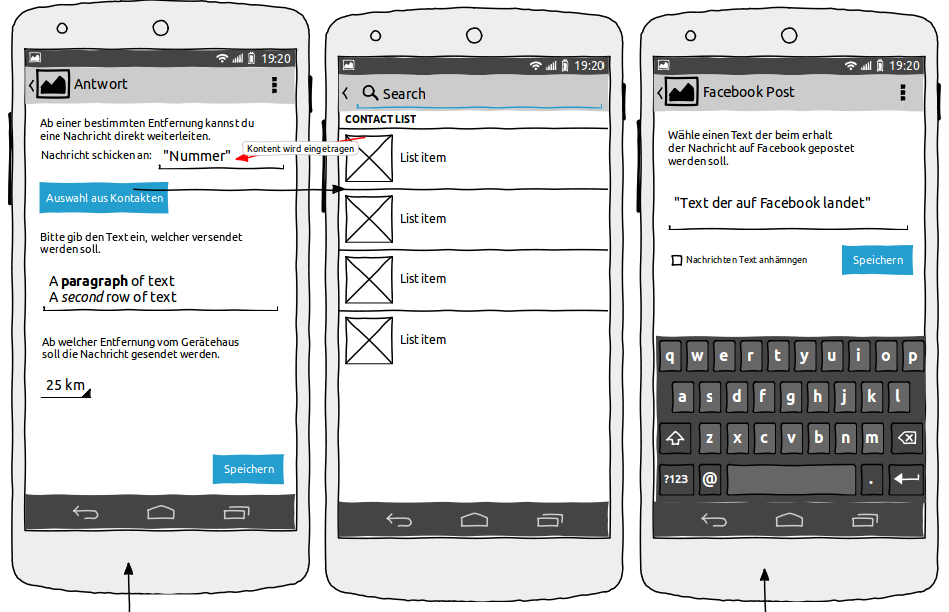
\includegraphics[width=16cm]{Bilder/WireframeAntwort.png}
\caption{Wireframe der automatisierten Antwort und des Facebookposts}
\label{Wireframe Antwort}
\centering
\end{figure}

\FloatBarrier
\begin{wrapfigure}{l}{5cm}
\vspace{-13pt}
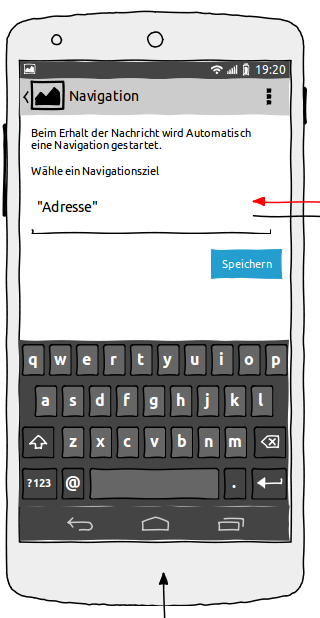
\includegraphics[width=5cm]{Bilder/WireframeNaviAuswahl.png}
\caption{Wireframe der Navigationsauswahl}
\label{Wireframe NaviAuswahl}
\vspace{-230pt}
\end{wrapfigure}
Im Bild \ref{Wireframe NaviAuswahl} ist die Activity zum einstellen eines Navigatinsziels zu sehen. Hier besteht zu einen die M\"oglickeit eine Adresse Selbstst\"andig einzugeben oder mit automatischer Google Erg\"anzung. Ist eine Adresse gew\"ahlt, muss der Nutzer diese wie schon \"ofter erl\"autert mit dem Speichern-Button sichern.

Hiermit wurden nun alle Activitys und M\"oglichkeiten dargestellt, die eine Regelerstellung bietet.
\newpage

\begin{wrapfigure}{l}{10cm}
\vspace{-13pt}
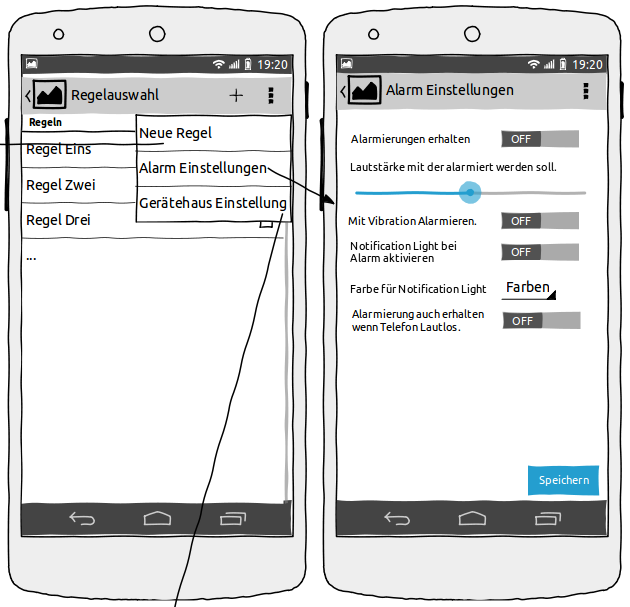
\includegraphics[width=10cm]{Bilder/WireframeRegeluebersicht_popup.png}
\caption{Wireframe der Regel\"ubersicht mit Popup und Alarmeinstellungen}
\label{Wireframe Regeluebersicht Popup}
\vspace{-20pt}
\end{wrapfigure}
Im Bild \ref{Wireframe Regeluebersicht Popup} links, ist wieder die Regelauswahl zu sehen, diesmal jedoch mit ge\"offnetem Popup-Men\"u. Das Men\"u enth\"alt die drei Punkte Neue Regel, Alarmeinstellungen und Ger\"atehauseinstellung. Der erste Men\"upunkt f\"uhrt wieder zu der Regelerstellung wie oben schon beschrieben. 

Der zweite Punkt \"offnet das globale Einstellungsmen\"u f\"ur den Alarmempfang, dies ist im Wireframe rechts dargestellt. Als erstes ist ein Schalter f\"ur die Aktivierung der Alarmierung zu finden. Ist dieser deaktiviert, so werden keine Alarme angezeigt. Als n\"achstes kann der Nutzer die Lautst\"arke des Alarms \"uber den Schieberegler ausw\"ahlen. Dies regelt die Lautst\"arke mit welcher ein Alarm angeben wird.

Als n\"achstes folgt der Schalter, an dem eingestellt werden kann, ob ein Alarm mit Vibration oder ohne signalisiert werden soll. Darauf folgt wieder ein Schalter, der das Notification Light bei einer Alarmierung aktiviert. Hierf\"ur gibt es nat\"urlich direkt darunter eine Auswahl der Lichtfarbe, mit der Alarmiert werden soll.

Der letzte Schalter ist der wahrscheinlich wichtigste, denn er gibt an ob eine Alarmierung auch erfolgen soll, wenn das Telefon sich im Lautlosenmodus befindet.

\begin{wrapfigure}{r}{5cm}
\vspace{-13pt}
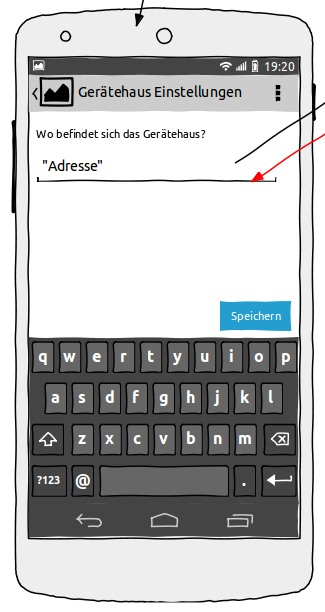
\includegraphics[width=5cm]{Bilder/WireframeGeraetehaus.png}
\caption{Wireframe der Ger\"atehauseinstellung}
\label{Wireframe Geraetehaus}
\vspace{-250pt}
\end{wrapfigure}
Die letzte noch fehlende Activity ist im Wireframe im Bild \ref{Wireframe Geraetehaus} zu sehen. In diese Activity gelangt man \"uber den dritten Popupmen\"upunkt. Die Activity enth\"alt einzig ein Textfeld, in das der Standort des Ger\"atehauses mit Hilfe der Google-Autovervollst\"andigung eingetragen werden kann.

Mit diesem Standort errechnet die App sp\"ater die Entferung zum Ger\"atehaus.
\newpage


\subsection{Die Evaluierung}

\subsection{Die Wireframes nach der Evaluierung}

\subsection{Auswirkungen der Evaluierung auf das Lastenheft}